\section{Introduction} \label{sec:introduction}

% /Users/zhangwenqian/Library/CloudStorage/Dropbox/应用/Overleaf/Nuclear CD/figure/graph.png

Graphs are fundamental data structures consisting of vertices and edges that model relational information. They are widely used across diverse domains, including social network analysis, bioinformatics, and knowledge graph modeling.
%
Beyond pairwise relations, higher-order structures such as cliques and nuclei often provide deeper insights into the underlying organization of networks, revealing cohesive communities and latent functional modules~\cite{luo2019higher,rossetti2019community}.
%
In social networks, cliques capture tightly connected friendship groups~\cite{leskovec2016snap,ugander2018structural}; in biological systems, dense patterns correspond to protein-protein interactions and functional complexes~\cite{luo2019higher}; in collaboration networks, they represent research groups formed through co-authorship~\cite{xia2017measuring,chen2019linking}; and on the World Wide Web, hyperlinks induce dense subgraphs corresponding to related content or topical communities~\cite{malliaros2013clustering,gibson1998inferring}.


Decomposing graphs into hierarchically cohesive substructures is a fundamental task in graph mining to understand complex network, enabling diverse applications such as community detection \cite{girvan2002community}, influence propagation \cite{kempe2003maximizing}, anomaly detection \cite{akoglu2015graph}, graph visualization \cite{huang2014graph}, and protein modeling \cite{sharan2006modeling}.
%
Common graph decomposition models include the $k$-core~\cite{malliaros2020core2,batagelj2011fast} and $k$-truss~\cite{huang2014triangle,zhu2021efficient}, which recursively peel away low-degree vertices or edges to expose progressively denser subgraphs.
% 
To better capture higher-order dense structures, \textit{nucleus decomposition} was introduced~\cite{firstNucleus}, providing finer granularity that uncovers progressively denser and more cohesive subgraphs in real-world networks.
%
It generalizes classical models such as $k$-core and $k$-truss by defining cohesiveness in terms of $r$-cliques and their participation in larger $s$-cliques, and can be naturally extended to other higher-order structures.


Specifically, given two integers $0 < r < s$, an $(r,s)$-nucleus is defined as a maximal subgraph in which every $r$-clique participates in at least $k$ distinct $s$-cliques (and all such $r$-cliques are $s$-connected).
%
The nucleus core number $\kappa_s(R)$ of an $r$-clique $R$ is defined as the maximum $k$ such that $R$ belongs to a $k$-$(r,s)$-nucleus.
%
This generalization subsumes classic notions: the $(1,2)$-nucleus corresponds to the $k$-core~\cite{seidman1983network}, the $(2,3)$-nucleus corresponds to the $k$-truss~\cite{cohen2008trusses}, while higher-order $(r,s)$ values yield clique-based, richer structural representations of network cohesiveness.

\begin{figure}[t]
    \centering
    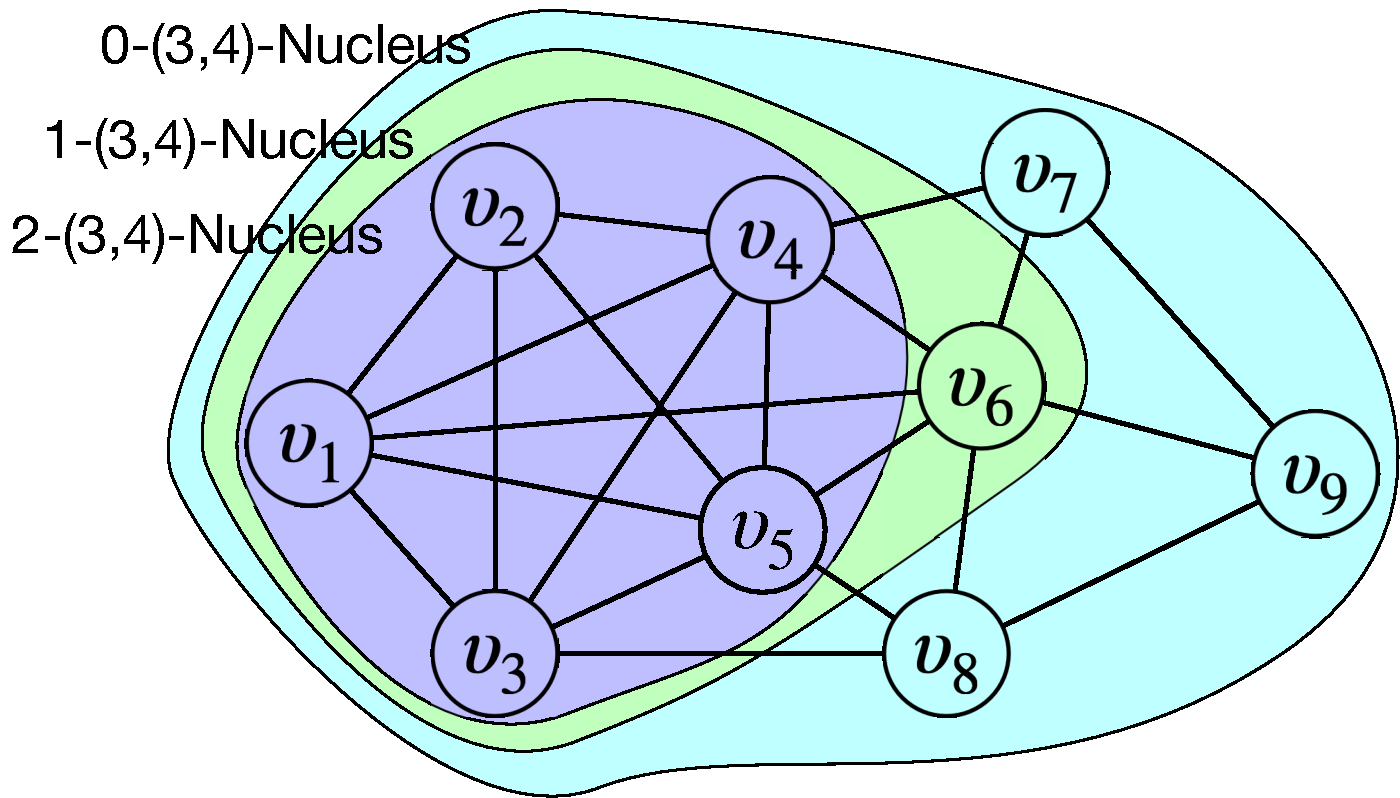
\includegraphics[width=0.32\textwidth]{figure/graph-eps-converted-to.pdf}
    \caption{An example of a graph $G$.}
    \label{fig:graph_example}
\end{figure}

\begin{example}
    Figure~\ref{fig:graph_example} illustrates a sample graph $G$. 
    Taking the $(3,4)$-nucleus as an example, the subgraph induced by vertices $v_1$, $v_2$, $v_3$, $v_4$, and $v_5$ forms a $2$-$(3,4)$-nucleus, as each $3$-clique is contained in at least two $4$-cliques. 
    For instance, the $3$-clique $(v_1, v_2, v_3)$ belongs to the $4$-cliques $(v_1, v_2, v_3, v_4)$ and $(v_1, v_2, v_3, v_5)$. 
    Similarly, all other $3$-cliques in this subgraph satisfy this condition. 
    The maximum nucleus core number for the $(3,4)$-nucleus in this graph is $2$.

    
    % In this graph, we can identify various cliques and analyze their participation in larger cliques to determine the $(r,s)$-nucleus. For instance, the triangle formed by vertices $v_1$, $v_2$, and $v_3$ is a $3$-clique, and we can explore how many $4$-cliques it participates in to compute its nucleus core number. 
    % % 在这个图中, 最大的k-(3,4)-nucleus是由顶点v1, v2, v3, v4, v5组成的2-(3,4)-nucleus, 因为每个3-团都至少包含在2个4-团中. 例如, 3-团(v1, v2, v3)包含在4-团(v1, v2, v3, v4)和(v1, v2, v3, v5)中. 类似地, 其他的3-团也满足这个条件. 因此, 这个图的k-(3,4)-nucleus的核数是2.
    % In this case, the largest $k$-$(3,4)$-nucleus consists of vertices $v_1$, $v_2$, $v_3$, $v_4$, and $v_5$, forming a $2$-$(3,4)$-nucleus since each $3$-clique is contained in at least two distinct $4$-cliques. For example, the $3$-clique $(v_1, v_2, v_3)$ is part of the $4$-cliques $(v_1, v_2, v_3, v_4)$ and $(v_1, v_2, v_3, v_5)$. Similarly, other $3$-cliques in this subgraph also satisfy this condition. Therefore, the nucleus core number for this graph's $k$-$(3,4)$-nucleus is $2$.
\end{example}


% \stitle{Applications.}
% Compared with coherent subgraph models such as the $k$-core and $k$-truss, the $(r,s)$-nucleus provides a more general higher-order model, where $(r,s)$ control cohesiveness. 
% %
% In co-authorship networks, nuclei reveal author groups whose triads repeatedly co-appear in larger cliques, indicating stable collaborations~\cite{newman2001structure,lu2016vital}. 
% %
% In social networks, nuclei highlight tightly knit interaction rings that require multi-actor closure, complementing existing community detection methods~\cite{girvan2002community,ugander2012structural}. 
% %
% In protein-protein interaction and functional networks, nucleus decomposition isolates near-clique modules consistent with biological complex formation~\cite{sharan2006modeling,luo2019higher}. 
% %
% In hyperlink and citation graphs, it identifies cohesive topical clusters~\cite{gleich2012graph,malliaros2013clustering}.


\stitle{Applications.}
% 
Compared with coherent subgraph models such as the $k$-core and $k$-truss, the $(r,s)$-nucleus provides a more general higher-order model, where $(r,s)$ control cohesiveness. 
\myaddRA{
% 
In particular, $r$ specifies the base clique unit, while $s$ specifies the cohesiveness of the resulting nuclei and thus how tightly connected they are.
% 
A larger $s$ imposes a stricter support requirement: an $r$-clique must participate in many distinct $s$-cliques, so nuclei persist only when higher-order overlap is abundant rather than accidental, providing stronger evidence of cohesion~\cite{firstNucleus}.
This requirement arises naturally in many domains; we discuss representative examples below:

% Compared with cohesive subgraph models such as $k$-core and $k$-truss, the $(r,s)$-nucleus is a more general higher-order model in which $r$ selects the base clique unit and $s$ controls the cohesiveness of the resulting nuclei.
% \myaddRA{
% A larger $s$ helps rule out incidental structures by retaining only regions where many $r$-cliques are repeatedly supported by larger clique closures, providing stronger corroboration of cohesion~\cite{firstNucleus}.
% This requirement arises naturally in many domains; we discuss representative examples below:


\sstitle{Coordinated fraud / collusion.}
From interaction logs, we can build a graph where suspicious accounts tend to act in lockstep on many targets.
High-$s$ nuclei help isolate small coordinated rings by filtering out casual triangles and keeping only groups with repeated multi-way coordination~\cite{beutel2013copycatch,hooi2016fraudar}.

\sstitle{Recommendation / e-commerce.}
In an item-to-item graph from co-purchase or co-click signals, high-$s$ nuclei highlight compact bundles of items that co-occur again and again across many users, which can be used as stable and interpretable bundles for browsing, diversification, or cold-start organization~\cite{linden2003amazon}.

\sstitle{Collaboration analysis.}
In a coauthor graph, high-$s$ nuclei capture stable teams whose collaborations are supported by many different higher-order coauthorship cliques, instead of being connected only through one large paper or a single hub author~\cite{newman2001structure}.

% Finally, increasing $r$ is most suitable when the application explicitly requires a minimum mutually connected group size, whereas increasing $s$ controls whether such a group is \emph{repeatedly} corroborated by higher-order interactions~\cite{firstNucleus}.
}


% The parameters $(r,s)$ act as design knobs—$r$ defines the anchor pattern and $s$ specifies the closure requirement—allowing cohesiveness to be tuned to domain semantics. 
%
% These examples illustrate scenarios where higher-order closure, rather than simple pairwise connectivity, is the key structural quantity of interest.
%
%  our counting-based framework enables such analyses at scale without materializing $K_s$.
% The $(r,s)$-nucleus decomposition provides a unifying framework that generalizes classical $k$-core and $k$-truss models, and serves as a foundation for analyzing higher-order structures in large-scale networks~\cite{firstNucleus,seidman1983network,cohen2008trusses}. Its applications span a wide range of domains. In scientific collaboration networks, vertices represent authors and cliques correspond to co-authorship groups. Nuclear decomposition reveals cohesive research communities and identifies influential collaborators~\cite{newman2001structure,lu2016vital}, highlighting long-term, stable collaborations that go beyond simple publication counts. Also, in online social networks, nucleus decomposition uncovers tightly knit groups, key influencers, and hidden community hierarchies~\cite{girvan2002community,ugander2012structural}. By focusing on higher-order structures rather than pairwise interactions, it improves the detection of strong, frequent interactions and enhances the analysis of influence propagation and anomaly detection~\cite{akoglu2015graph}. Similarly, in biological networks, $(r,s)$-nuclei capture protein complexes, metabolic pathways, and functional modules, offering a more accurate representation of molecular interactions than pairwise methods~\cite{sharan2006modeling,luo2019higher}. This enables the discovery of biologically meaningful structures that drive cellular functions. In addition, in the World Wide Web and information networks, nucleus decomposition identifies dense hyperlink-induced subgraphs that represent coherent topical communities~\cite{gleich2012graph, malliaros2013clustering}. These insights can improve web mining, content recommendation, and spam detection by distinguishing interlinked pages from sparse connections.  

% More broadly, nucleus decomposition supports applications in \textbf{network visualization}, where hierarchical dense structures aid in scalable layout design~\cite{huang2014graph}, in \textbf{densest subgraph discovery}~\cite{tsourakakis2013finding}, and in \textbf{network security}, where dense interaction patterns reveal coordinated malicious behaviors~\cite{jiang2016catching}. A particularly important direction is the \textbf{real-time analysis of billion-scale networks}, such as transaction graphs in financial systems, large-scale communication records, or knowledge graphs containing billions of entities and relations. Traditional peeling-based or $h$-index-based frameworks cannot operate in these settings, since explicit enumeration of $s$-cliques or repeated updates of all $r$-cliques are computationally infeasible and memory intensive. Our counting-based framework directly addresses this gap. By replacing clique enumeration with a succinct counting process, it reduces the computational overhead to a scale where continuous updates are possible. The Succinct Clique Tree (SCT) representation compactly encodes the clique space, making support computation feasible even when the underlying graph contains billions of vertices and edges. Furthermore, the framework achieves memory efficiency by avoiding pre-computed clique indices, ensuring that the memory footprint grows linearly with graph size rather than exponentially with clique order. Parallelization further enables decomposition to keep pace with streaming data, which is critical for real-time monitoring.  

% To illustrate, consider a \textbf{financial transaction network} where vertices represent accounts and edges represent money transfers. Higher-order dense subgraphs in this graph may correspond to tightly coordinated transaction groups, which are strong indicators of money laundering, fraudulent trading, or collusive market behavior. In such networks, the volume of daily transactions can reach billions, and new data arrives continuously. Existing decomposition methods cannot scale to this volume, let alone provide timely detection. Our counting-based approach enables the identification of $(r,s)$-nuclei that highlight suspicious clusters in near real time, allowing regulators and financial institutions to react to illicit activities as they occur rather than after significant delays. This scenario demonstrates both the scalability and the practical importance of our framework: it transforms nucleus decomposition from a purely theoretical model into a tool capable of addressing pressing challenges in massive real-world networks.

\stitle{Existing Methods and Key Limitation.} 
Despite its effectiveness and broad applicability, computing nucleus decomposition is computationally intensive, motivating extensive research on improving its efficiency~\cite{sotaHierarchy,sotaPrveHierarchy,LocalNuclear,firstNucleus,nuclearTWEB,nuclearcsonet20}. 
%
Existing studies primarily focus on optimizing the peeling process~\cite{sotaPrveHierarchy,sotaHierarchy}, where the key idea is to iteratively remove low-support $r$-cliques those that participate in fewer $s$-cliques to expose progressively denser substructures. 
%
Other lines of research explore parallel acceleration, either through local update strategies~\cite{LocalNuclear} or multi-threaded peeling algorithms~\cite{sotaPrveHierarchy,sotaHierarchy}. 


However, all existing algorithms share a fundamental limitation: they rely on explicit \textbf{\textit{clique enumeration}}, requiring all $s$-cliques in the graph to be enumerated. 
%
Such enumeration significantly limits scalability, as the number of $s$-cliques increases combinatorially with $s$, often reaching trillion scale even for moderate values of $s$. 
%
As a result, existing approaches are typically limited to small parameter settings (e.g., $(3,4)$-nucleus) or to small and sparse graphs.
%
In theory, the best existing methods achieve asymptotic work complexity comparable to full $s$-clique enumeration~\cite{sotaPrveHierarchy,sotaHierarchy}, leaving the intrinsic computational barrier of explicit clique listing unresolved, particularly for larger graphs and higher parameter values.

% \begin{figure}[t]
%   \centering
%   \begin{subfigure}[b]{0.45\linewidth}
%     \includegraphics[width=\linewidth]{figure/clique_distribution_dblp.eps}
%     \caption{DBLP}
%   \end{subfigure}
%   % \hfill
%   \begin{subfigure}[b]{0.45\linewidth}
%     \includegraphics[width=\linewidth]{figure/clique_distribution_stanford.eps}
%     \caption{web-Stanford}
%   \end{subfigure}
%     \caption{The distribution of $k$-cliques in the datasets. 
%     % The x-axis represents the size of the clique, and the y-axis represents the number of cliques of that size.
%     }
%     \label{fig:clique_distribution}
% \end{figure}

\begin{example}
    The number of $k$-cliques grows explosively with increasing $k$. 
    % Figure~\ref{fig:clique_distribution} shows the clique distribution on the \textsc{DBLP} and \textsc{Stanford} datasets (in Table~\ref{tab:graph-stats}). 
    We observe that in \textsc{DBLP}, the number of $6$-cliques already exceeds $4\times10^9$ and reaches $1.5\times10^{36}$ at $k{=}57$; in \textsc{web-Stanford}, it includes $2.2\times10^{12}$ $28$-cliques.
    Because existing frameworks explicitly enumerate $s$-cliques, the computation becomes quickly infeasible—even enumerating all $6$-cliques alone incurs substantial overhead(Figure \ref{fig:leafcount}).
\end{example}

% The problem is NP-complete, making it challenging to apply to large graphs. Nevertheless, due to its effectiveness and broad applicability, 

% The two prevailing paradigms are: (i) peeling-based methods~\cite{shan2018finding,montresor2013distributed}, which iteratively remove the least-supported $r$-cliques until all remaining satisfy the nucleus condition; and (ii) local $h$-index-based methods~\cite{firstNucleus}, which iteratively update nucleus core numbers by examining neighborhoods of $s$-cliques. While peeling is efficient for small clique sizes, its complexity scales directly with $|K_s|$, the number of $s$-cliques, which is infeasible in practice. The $h$-index method avoids global peeling but requires multiple rounds of iterative updates, each involving expensive neighborhood checks. Both frameworks fundamentally depend on enumerating all $s$-cliques, which prevents them from handling larger $r,s$ values or billion-scale graphs.

\stitle{Research Question.} 
This leads to the critical research question and the main objective of this paper: \textbf{\textit{How to compute $(r,s)$-nucleus decomposition without explicitly enumerating $s$-cliques?}}

\stitle{Challenges.} 
Avoiding $s$-clique enumeration in nucleus decomposition is highly challenging, as enumeration is deeply embedded in all existing algorithmic frameworks.
%
All existing algorithms rely on explicitly enumerating all $s$-cliques for three essential reasons:

% \begin{enumerate}[leftmargin=*]
%     \item \textbf{Computing the support of each $r$-clique:} determining how many $s$-cliques each $r$-clique participates in.
%     \item \textbf{Updating neighboring $r$-cliques during peeling:} when an $r$-clique is removed, the supports of its adjacent $r$-cliques must be updated, which requires access to the shared $s$-cliques.
%     \item \textbf{Defining connectivity between $r$-cliques for hierarchy construction:} hierarchical structures are built based on shared $s$-cliques, again necessitating enumeration.
% \end{enumerate}


\sstitle{Computing the support of each $r$-clique.} 
%
The support of an $r$-clique $R$ is defined as the number of $s$-cliques containing it. 
Existing methods compute this by enumerating all $s$-cliques and recording, for each $r$-clique, the set of $s$-cliques that include it.

\sstitle{Updating neighboring $r$-cliques during peeling.} 
When an $r$-clique $R$ is removed during the peeling process (along with all $s$-cliques containing it), every $r$-clique $R'$ that shares an $s$-clique with $R$ must have its support decremented by $1$. 
This update requires knowing, for each $s$-clique, the set of $r$-cliques it contains; thus, adjacency among $r$-cliques is derived from enumerated $s$-cliques.

\sstitle{Defining connectivity for hierarchy construction.}
%
Two $r$-cliques $R$ and $R'$ are \emph{$s$-connected} if a sequence of $r$-cliques exists such that each consecutive pair of cliques shares at least one common $s$-clique. 
To identify nucleus components for hierarchy construction, existing algorithms enumerate and traverse all $s$-cliques to determine these connectivity relationships.


% However, all existing approaches share a fundamental limitation: they are \textbf{enumeration-based}, requiring explicitly enumerating all $s$-cliques in the graph. This significantly restricts their scalability to large graphs and higher value of $s$.
% % \todo{why do existing methods enumerate s-cliques? why is it (\textbf{fundamentally}) hard to compute $(r,s)$-nucleus without enumeration? }
% % Unlike pairwise cores where degrees provide simple update rules, nucleus decomposition requires enumerating all $s$-cliques to compute the $(r,s)$-support of each $r$-clique. 
% Exact $(r,s)$-support for an $r$-clique equals the number of $s$-cliques containing it. Without a counting oracle, the only general way to obtain and maintain these supports during peeling is to materialize (or re-enumerate) the incident $s$-cliques. Supports are not functions of local degrees: an $r$-clique can form $s$-cliques through many overlapping, non-local neighborhoods, so deletions propagate widely. Hence existing frameworks reduce exact maintenance to listing or indexing $K_s$, which leads to combinatorial blow-up as $s$ increases.

% Unlike pairwise cores where degrees provide simple update rules, nucleus decomposition requires enumerating all $s$-cliques to compute the $(r,s)$-support of each $r$-clique. 
 
% We identify three major bottlenecks:

% \sstitle{Clique enumeration overhead.}  
% A principal difficulty arises from the reliance on enumerating all $s$-cliques in order to compute the support of each $r$-clique. Since the number of $s$-cliques grows combinatorially with graph size and clique order, this step dominates the runtime of existing algorithms. The enumeration overhead fundamentally restricts scalability and makes nucleus decomposition infeasible for large graphs or higher-order parameters. Overcoming this challenge is crucial to enable algorithms that avoid explicit enumeration and can operate efficiently on complex networks.  

% \sstitle{Inefficient counting maintenance.}  
% The core difficulty is not maintaining the cliques themselves, but maintaining the \emph{counting} of $s$-cliques per $r$-clique as the decomposition progresses. When one $r$-clique is removed, every $s$-clique containing it becomes invalid, and consequently the counting of all other $r$-cliques in those $s$-cliques must be decremented. Existing approaches attempt to handle this either by re-enumerating affected $s$-cliques\cite{fastHierarchy,LocalNuclear}, which causes massive redundancy and wasted computation, or by storing explicit mappings from each $r$-clique to all of its incident $s$-cliques, which requires frequent updates. Neither approach provides a scalable solution. Current frameworks therefore lack a compact, update-friendly representation that can deliver correct support deltas without exhaustive neighborhood scans. Overcoming this limitation is critical, since accurate and selective maintenance of counting is the prerequisite for enabling nucleus decomposition to scale to large graphs and higher-order parameters.

% \sstitle{Lack of hierarchical exploitation.}  
% Nuclear decomposition is inherently hierarchical: an $(r,s)$-nucleus is nested within higher-order structures, and computing deeper levels of the decomposition depends on accurate values at shallower levels. Existing algorithms cannot fully exploit this hierarchy, because their reliance on enumeration and updates prevents reusing intermediate results across levels. Thus, they recompute supports from scratch for each stage, incurring exponential computation time. The inability to maintain and propagate hierarchical information has been a critical bottleneck in applying nucleus decomposition to large, complex graphs. 

\stitle{Our Idea.} 
% Inspired by the advances in clique counting~\cite{Pivoter}, 
To efficiently support the above core operations of nucleus decomposition while avoiding explicit $s$-clique enumeration, we design a novel auxiliary data structure, the \textit{Clique Path Index} (\cpi), 
%
% maximial clique enumeration should be mentioned somewhere?
\cpi encodes the space of $s$-cliques into compact paths, enabling counting, updates, and connectivity queries to be executed directly over these paths without enumeration. 
%
The proposed index provides the following key features:

\sstitle{Counting without enumeration.} 
%
\cpi enables $s$-clique counting and the computation of $r$-clique supports by aggregating path statistics, thereby avoiding the exponential overhead of enumerating all $s$-cliques as in existing algorithms.

\sstitle{Dynamic and efficient updates.} 
%
\cpi performs efficient incremental updates during peeling by dynamically modifying or splitting affected clique paths upon deletions.
As clique information is aggregated in the path representation, removing a single $r$-clique implicitly accounts for the removal of many $s$-cliques, thereby significantly reducing redundant computation during peeling.

\sstitle{Built-in connectivity maintenance.} 
%
\cpi maintains $s$-connectivity naturally among $r$-cliques during updates. 
Connectivity relationships are preserved and adjusted within the indexed paths, enabling hierarchy construction to be performed directly without additional traversal or re-enumeration.

\sstitle{From index design to differential maintenance.}
%
While \cpi resolves the representation problem, the remaining algorithmic challenge is how to maintain exact supports during peeling without reverting to local re-materialization.
%
Our journal-level view is that nucleus peeling on \cpi is fundamentally a \emph{differential path contribution maintenance} problem:
each path contributes a local amount of support to the $r$-cliques it covers, and after a peeling round only the contributions on paths incident to removed $r$-cliques can change.
%
This perspective isolates the true source of efficiency gains beyond the index itself and explains why different regimes of $r$ admit different exact update mechanisms.


% 1. Computing the Support of Each $r$-Clique -> counting
% 2. Updating Neighboring $r$-Cliques (during the Peeling Process) -> remove redundant computation
% 3. Defining Connectivity Between $r$-Cliques (Hierarchy Construction) -> filtering 


\stitle{Contributions.} 
Building on the proposed \textit{Clique Path Index} (\cpi), we present a counting-based nucleus decomposition framework.
%
We also present a higher-level differential maintenance theory for exact peeling.
%
The main contributions of this work are summarized as follows:

\sstitle{Counting-based nucleus decomposition via the Clique Path Index.}
%
We propose a compact path-based representation of the $s$-clique search space that avoids explicit $s$-clique enumeration while still supporting exact support counting, dynamic updates, and hierarchy construction.
%
This is the representation layer of our method.

\sstitle{A differential path contribution maintenance theory.}
%
We formalize nucleus peeling on \cpi as maintaining path-local support contributions under deletions.
%
Under this view, the support of each active $r$-clique is the sum of path contributions.
%
After each peeling round, only paths incident to removed $r$-cliques need updates.

\sstitle{Exact regime-specific update operators for $r{=}1$, $r{=}2$, and $r{\ge}3$.}
%
Under the differential maintenance view, we derive three exact specialized instantiations:
counter-only path maintenance for $r{=}1$,
closed-form deltas and analytical single-edge splits for $r{=}2$,
and dead-path-aware lazy maintenance for $r{\ge}3$.
%
These instantiations show how the same framework leads to different update operators in different regimes.

\sstitle{Integrated hierarchy construction and comprehensive evaluation.}
%
Our method naturally preserves $s$-connectivity among $r$-cliques within \cpi, enabling hierarchy construction with minimal extra overhead.
%
Experiments show clear gains over prior methods.
%
On comparable settings, our method is about $4\times$ faster than \arb and about $13\times$ to $27\times$ faster than the \nucleus baselines.
%
On some instances, the speedup exceeds two orders of magnitude.
%
The gains hold for both decomposition and hierarchy construction.

\sstitle{Extension over the conference version.}
%
Compared with the conference version of this work, this journal version makes three substantive extensions.
%
First, it introduces the differential path contribution maintenance formalism.
%
This formalism isolates the exact support-update primitive beyond the index itself.
%
Second, it derives regime-specific sufficient states and exact update operators for $r{=}1$, $r{=}2$, and $r{\ge}3$.
%
These operators follow one common maintenance principle.
%
Third, it strengthens the optimization and complexity analysis.
%
It explains how different peeling regimes reduce update costs without losing exactness.

\stitle{Organization.}
%
Section~\ref{sec:preliminaries} reviews the problem definition and notation.
%
Section~\ref{sec:existing_approaches} revisits the peeling baseline and motivates avoiding explicit $s$-clique enumeration.
%
Section~\ref{sec:our_approach} introduces the representation layer through \cpi.
%
Section~\ref{sec:dpcm} then lifts it to a differential path contribution maintenance view.
%
Section~\ref{sec:update_cpi} then instantiates this view for general $r{\ge}3$, for $r{=}2$, and for $r{=}1$, followed by dead-path-aware refinements.
%
The remaining sections present hierarchy construction, experiments, case studies, and related work.


% 

% All prior algorithms for nucleus decomposition have been tied to explicit enumeration, either constructing every $s$-clique in advance or re-enumerating them during updates. This reliance on enumeration has been the fundamental scalability barrier, as the number of $s$-cliques grows combinatorially with graph size and clique order. We present the first \emph{counting-based} framework for nucleus decomposition, which replaces explicit enumeration with direct clique-counting operations over the Succinct Clique Tree (SCT). This breakthrough eliminates the exponential dependence on $s$-clique enumeration and allows supports to be computed and maintained in closed form. As a result, our framework makes it possible, for the first time, to perform nucleus decomposition at higher-order parameters and on graph scales that were previously infeasible. This shift from enumeration to counting marks a fundamental change in how nucleus decomposition is designed and establishes a new foundation for scalable higher-order graph analysis.


% \sstitle{First efficient update mechanism.}
% Prior algorithms for nucleus decomposition lacked any practical way to maintain support counts incrementally. They relied on recomputation or full re-enumeration of affected cliques, which introduced massive redundancy and prevented scalability. We provide the first efficient update mechanism by leveraging the Succinct Clique Tree (SCT) together with clique-counting formulas and pruning strategies. This mechanism updates supports selectively and maintains the tree incrementally, avoiding reconstruction of local substructures. As a result, nucleus decomposition is no longer bound to costly iterative recomputation but can instead be performed with efficient, scalable updates, making the method practical for massive real-world graphs.

% \sstitle{Succinct data structure for counting.}  
% Existing algorithms for nucleus decomposition lack any data structure that can maintain clique counts compactly and update them efficiently. The state-of-the-art methods either re-enumerate all affected cliques after every deletion, incurring prohibitive overhead, or store explicit mappings from each $r$-clique to its incident $s$-cliques, which quickly becomes infeasible in memory. We introduce the first SCT-based data structure that encodes the entire clique space in a compressed, lossless representation. This structure supports direct counting of $s$-cliques containing any $r$-clique without explicit enumeration, and it enables incremental updates during decomposition without scanning large neighborhoods. By combining compactness with update efficiency, the SCT data structure resolves a long-standing bottleneck in nucleus decomposition: how to maintain counting information at scale. This innovation provides the theoretical foundation and practical backbone that makes our counting-based framework possible, and represents a significant departure from all previous approaches.
 

% \sstitle{Hierarchy without prior knowledge of $s$.} \ A key advantage of our framework is that it can compute the full hierarchy of nucleus structures without requiring $s$ to be fixed in advance. Existing state-of-the-art methods typically recompute supports separately for each choice of $s$, which is costly and inflexible. By contrast, our approach leverages the Succinct Clique Tree (SCT) representation to decide $s$-connectivity. This property allows us to identify nuclei hierarchically across all possible values of $s$ in a unified manner. To maintain this hierarchy efficiently during decomposition, we employ a multi-level disjoint set union (DSU) structure in which each level corresponds to a $k$-core. This design ensures that once two $r$-cliques are merged at a given level, they remain merged in all smaller levels, thereby preserving containment relationships. As a result, our framework constructs the entire nucleus hierarchy dynamically and incrementally, eliminating the need for recomputation at different values of $s$. This capability is crucial for large-scale analysis, as it enables flexible exploration of higher-order structures even when the appropriate $s$ is not known beforehand.





% \sstitle{Comprehensive experimental validation.}  
% We conduct an extensive set of experiments on real-world datasets of varying scale and density. Our work advances the state-of-the-art by moving beyond previous time-outs, enabling efficient computation and obtaining results on comparatively large graphs. These improvements validate the effectiveness of our framework across different application domains. They show that our approach not only advances the theoretical state-of-the-art but also provides a practical solution that can be immediately applied in large-scale graph analysis.
